\documentclass[12pt,a4paper]{article}
\usepackage{commons/style}

\begin{document}

% =========================== Assignment Mode ============================

% --- Course Information ---
\coursetitle{هوش مصنوعی}
\semester{بهار 1405}
\prof{ماری‌اوریاد}

% --- Student Information ---
\studentname{محسن صلاح}
\studentid{403106238}

% --- Assignment Details ---
\assignmenttype{تمرین اول}
\assignmenttitle{جستجوی ناآگاهانه، آگاهانه و محلی}

\maketitle

% ========================================================================

\sectiontitle{سوالات نظری}

\question{}

\begin{ابجد}
\item \textbf{نادرست}؛ در جستجوی گرافی تمام گره‌هایی که قبلاً از آنها بازدید کرده‌ایم نیز ذخیره می‌شوند تا از بررسی مجدد آنها جلوگیری شود. بنابراین پیچیدگی فضایی\footnote{\lr{Space Complexity}} الگوریتم \lr{DFS} در این حالت از مرتبه $O(b^m)$ می‌باشد.

\item \textbf{درست}؛ طبق تعریف تابع اکتشافی $h$ یک‌نوا است اگر:
\[ \forall A, B: h(A) - h(B) \leq \mathrm{cost}(A \to B) \]
حال اگر دو تابع اکتشافی $h_1$ و $h_2$ یک‌نوا باشند، به سادگی می‌توان نتیجه گرفت که:
\begin{align*}
    h_1(A) - h_1(B) & \leq \mathrm{cost}(A \to B) \\
    h_2(A) - h_2(B) & \leq \mathrm{cost}(A \to B)
\end{align*}
با جمع دو رابطه بالا داریم:
\[ (h_1 + h_2)(A) - (h_1 + h_2)(B) \leq 2 \times \mathrm{cost}(A \to B) \]
با تقسیم طرفین بر $2$ نتیجه می‌شود:
\[ \forall A, B: \left(\frac{h_1 + h_2}{2}\right)(A) - \left(\frac{h_1 + h_2}{2}\right)(B) \leq \mathrm{cost}(A \to B) \]
بنابراین $\frac{h_1 + h_2}{2}$ یک تابع اکتشافی یک‌نوا است.

\item \textbf{نادرست}؛ مثال نقض می‌آوریم. فرض کنید به ازای تابع اکتشافی $h_1$ و دو گره $A$ و $B$ داریم:
\begin{align*}
    h_1(A)                 & = 3 \\
    h_1(B)                 & = 2 \\
    \mathrm{cost}(A \to B) & = 2
\end{align*}
می‌دانیم که $h_1$ یک‌نوا هست و رابطه $h_1(A) - h_1(B) \leq \mathrm{cost}(A \to B)$ صحیح می‌باشد. حال اگر عدد ثابت $c = 3$ را در نظر بگیریم:
\begin{align*}
    h_2(A) & = 9 \\
    h_2(B) & = 6
\end{align*}
اکنون داریم $h_2(A) - h_2(B) = 3 \nleq \mathrm{cost}(A \to B)$ و رابطه مورد نظر دیگر برای گره‌های $A$ و $B$ صادق نیست، پس تابع $h_2$ یک‌نوا نیست.

\item \textbf{درست}: می‌دانیم طبق تعریف به تابع اکتشافی‌ای قابل قبول\footnote{Admissible} گفته می‌شود که:
\begin{align*}
    \forall n, 0 \leq h(n) \leq h^*(n)
\end{align*}
که $h^*(n)$ هزینه واقعی است.
\begin{proof}
    فرض کنید دو هدف قابل دسترس $A$ و $B$ داریم که $A$ بهینه و $B$ غیر بهینه\footnote{suboptimal} است. $n$ یک جد دلخواه $A$ (شامل خود $A$) است؛ می‌خواهیم نشان دهیم که $n$ زودتر از $B$، از \lr{fringe} خارج می‌شود. از سه مورد زیر استفاده می‌کنیم:
    \begin{enumerate}
        \item $g(A) < g(B)$؛ چون $A$ هدف بهینه، و $B$ غیر بهینه است.
        \item $h(A) = h(B) = 0$؛ چون تابع $h$ قابل قبول است.
        \item $f(n) \leq f(A)$؛ به این شکل نشان داده می‌شود:
              \begin{align*}
                  h(n) \leq h^*(n) \Rightarrow & g(n) + h(n) \leq g(n) + h^*(n) \\
                  \Rightarrow                  & f(n) \leq g(A)                 \\
                  \xRightarrow{h(A) = 0}       & f(n) \leq f(A)
              \end{align*}
    \end{enumerate}
    اکنون از این سه مورد استفاده می‌کنیم:
    \begin{align*}
        \text{1 و 2} \Rightarrow g(A) + h(A) < g(B) + h(B)       \Rightarrow & f(A) < f(B)               \\
        \xRightarrow{\text{3}}                                               & f(n) < f(B) \quad (\star)
    \end{align*}
    چون از ابتدا فرض کرده بودیم که $n$ یک جد دلخواه $A$ (شامل خود $A$) هست، طبق رابطه ($\star$) نتیجه می‌گیریم که تمام اجداد $A$ از جمله خودش، پیش از $B$ بسط داده می‌شوند؛ پس نتیجه می‌گیریم که در این حالت الگوریتم $A^*$ بهینه است.
\end{proof}

\item \textbf{نادرست}؛ الگوریتم \lr{Local Beam Search} با $k=1$، همواره تمام همسایه‌های حالت فعلی را تولید کرده و سپس بهترین گزینه بین آنها را انتخاب می‌کند؛ بنابراین اگر تمام همسایه‌ها بدتر از حالت فعلی باشند، الگوریتم به ناچار بهترینِ آن‌ها را (که نسبت به حالت فعلی بدتر است) انتخاب می‌کند. \\
در مقابل الگوریتم \lr{Simulated Annealing} هر بار به طور تصادفی یکی از همسایه‌ها را انتخاب می‌کند: اگر این همسایه بهتر از حالت فعلی باشد، انتخاب می‌شود. اما اگر بدتر باشد، با احتمالی انتخاب می‌شود که این احتمال با کاهش دما کم می‌شود. به طور خلاصه هنگامی که دما به صفر میل می‌کند، الگوریتم \lr{SA} همسایه‌ای که بدتر از حالت فعلی باشد را انتخاب نمی‌کند، و از طرفی همسایه انتخاب شده هم لزوما «بهترین» همسایه ممکن نیست.

\item \textbf{نادرست}؛ الگوریتم \lr{BFS} در طول اجرای خود هر گره را حداکثر یک بار بسط می‌دهد. در مقابل، الگوریتم \lr{IDS} هر بار که حد عمق (\lr{limit}) جدیدی تعریف می‌کند، جستجو را مجدداً از ریشه درخت آغاز کرده و تمام گره‌های سطوح قبلی را دوباره بسط می‌دهد. \\
به همین دلیل، گره‌های سطوح بالاتر چندین بار (به عنوان مثال، گره ریشه $d+1$ بار) باز می‌شوند. در نتیجه، تعداد کل گره‌های بسط‌یافته در \lr{IDS} همواره اکیداً بیشتر از \lr{BFS} است (هرچند مرتبه مجانبی هر دو $O(b^d)$ می‌باشد).

\item \textbf{درست}؛ می‌دانیم که الگوریتم \lr{UCS} همواره گره با کمترین هزینه را از \lr{fringe} خارج می‌کند. حال اگر یال با هزینه 0 داشته باشیم، ممکن است الگوریتم در یک حلقه گیر کرده و هیچ گاه خاتمه نیابد. به عنوان مثال فرض کنید هم از گره $A$ به گره $B$ یال داریم و هم از گره $B$ به گره $A$، و هزینه هر دو یال نیز صفر است. همچنین فرض کنید در این مسئله هزینه تمام اکشن‌های دیگر بیشتر از صفر باشد. در این صورت اگر الگوریتم به یکی از این دو گره برسد، همواره یال با هزینه صفر را انتخاب می‌کند و هیچ گاه از این حلقه خارج نمی‌شود. \\
البته باید توجه کنیم که این مثال برای \lr{UCS} در حالت جستجوی درختی درست است. اگر بخواهیم از الگوریتم در جستجوی گرافی استفاده کنیم، از آنجا که در این حالت الگوریتم لیست گره‌های بسط داده شده را نگه می‌دارد (\lr{closed set}) امکان ندارد که در دوری با تعداد گره محدود گیر کند؛ در این روش تنها حالتی که امکان دارد گره در یک دور گیر کند، این است که یک دنباله از گره‌ها داشته باشیم که هزینه بین هر دو گره متوالی 0 باشد؛ در این صورت دیگر فضای مسئله متناهی نیست. (این موضوع منافاتی با صورت مسئله ندارد، چون ممکن است که در این فضا یک پاسخ متناهی داشته باشیم.)

\item \textbf{درست}؛ برای اثبات یک‌نوا بودن تابع اکتشافی $h$ باید نشان دهیم به ازای دو گره دلخواه \lr{A} و \lr{B}، که از \lr{A} به \lr{B} مسیری وجود داشته باشد:
\begin{align*}
    h(A) - h(B) \leq \mathrm{cost}(A \to B)
\end{align*}
یا به طور معادل:
\begin{align*}
    h(A) \leq \mathrm{cost}(A \to B) + h(B)
\end{align*}
\begin{proof}
    از یک‌نوا بودن $h_1$ و $h_2$ نتیجه می‌گیریم که به ازای هر دو گره دلخواه \lr{A} و \lr{B}، که از \lr{A} به \lr{B} مسیری وجود داشته باشد، داریم:
    \begin{align*}
        h_1(A) \leq \mathrm{cost}(A \to B) + h_1(B) \qquad & \text{(1)} \\
        h_2(A) \leq \mathrm{cost}(A \to B) + h_2(B) \qquad & \text{(2)}
    \end{align*}
    تابع اکتشافی $h = \min(h_1,h_2)$ را بررسی می‌کنیم.
    می‌دانیم که:
    \begin{align*}
        h(B) = h_1(B) \lor h(B) = h_2(B)        \qquad & \text{(3)} \\
        h(A) \leq h_1(A) \land h(A) \leq h_2(A) \qquad & \text{(4)}
    \end{align*}
    بنابراین:
    \begin{align*}
        \text{(4)} \xRightarrow{\text{(1) , (2)}} {\left\{\begin{aligned}
                                                                  h(A) \leq \mathrm{cost}(A \to B) + h_1(B) \\
                                                                  h(A) \leq \mathrm{cost}(A \to B) + h_2(B)
                                                              \end{aligned}\right.} \xRightarrow{\text{(3)}} h(A) \leq \mathrm{cost}(A \to B) + h(B)
    \end{align*}
    بنابراین تابع اکتشافی $h$ یک‌نوا است.
\end{proof}

\item \textbf{نادرست}: به طور کلی با افزایش $k$ در الگوریتم \lr{Local Beam Search} حالت‌های بیشتری بررسی می‌شوند و شانس گیر کردن در نقاط \lr{local maximum} یا نواحی \lr{flat} کمتر می‌شود. اما با افزایش $k$، تعداد همسایه‌هایی که باید در هر حالت محاسبه شوند نیز بیشتر می‌شود که در این حالت اجرای هر مرحله از الگوریتم مدت زمان بیشتری طول می‌کشد و ممکن است پیش از رسیدن به حالت هدف، زمان اجرای الگوریتم تمام شود. همچنین در هر مرحله باید همسایه‌های $k$ حالت فعلی ذخیره شوند تا بتوانیم $k$ تای بهتر را از بین آنها انتخاب کنیم. اگر تعداد همسایه‌ها خیلی زیاد شود، ممکن است به محدودیت حافظه بخوریم و الگوریتم متوقف شود.

\item \textbf{نادرست}: مثال نقض می‌آوریم. به این شکل توجه کنید:
\begin{latin}
    \begin{center}
        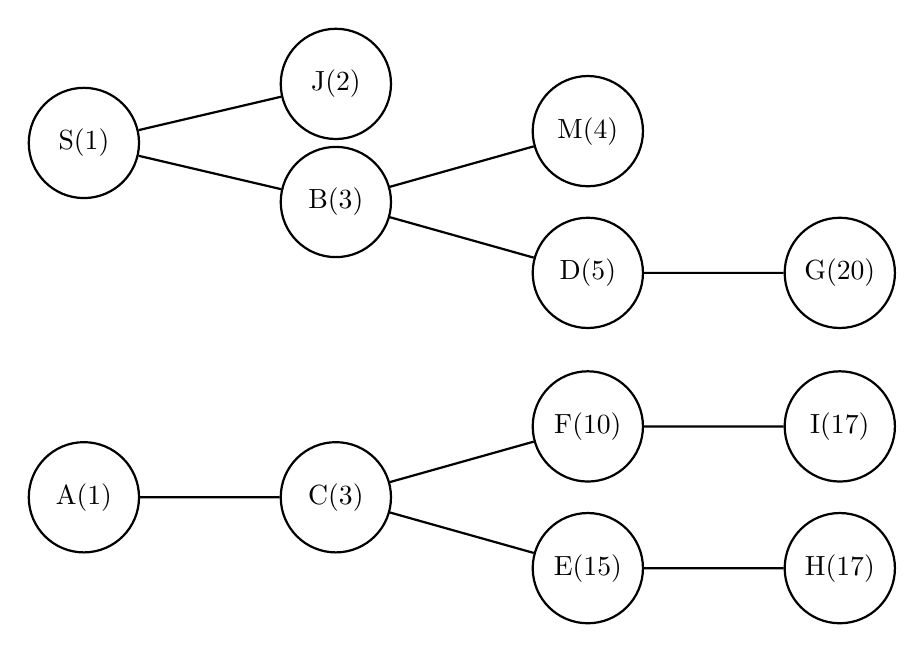
\begin{tikzpicture}[
                grow=right,
                level distance=3.2cm,
                level 2/.style={sibling distance=1.8cm},
                every node/.style={
                        draw, thick, circle,
                        minimum size=1.4cm,
                        inner sep=0pt,
                        align=center
                    },
                edge from parent/.style={draw, thick}
            ]

            \node at (0, 2) {S(1)}
            child {node {B(3)}
                    child {node {D(5)}
                            child {node {G(20)}}
                        }
                    child {node {M(4)}}
                }
            child {node {J(2)}};

            \node at (0, -2.5) {A(1)}
            child {node {C(3)}
                    % Bottom branch
                    child {node {E(15)}
                            child {node {H(17)}}
                        }
                    % Top branch
                    child {node {F(10)}
                            child {node {I(17)}}
                        }
                };

        \end{tikzpicture}
    \end{center}
\end{latin}
در این مثال هر گره، یکی از حالت‌های کامل\footnote{Complete} مسئله است و مقابل اسم هر یک، مقدار تابع \lr{fitness} به ازای آن نوشته شده. همچنین حالت‌های همسایه با یال به هم متصل شده‌اند. هدف، پیدا کردن حالت با بیشینه مقدار تابع \lr{fitness} است که در این مثال همان حالت $G$ می‌باشد. \\
در این مثال، الگوریتم \lr{Hill Climbing} با شروع از حالت $S$، به ترتیب به گره‌های $B$، $D$ و در نهایت به حالت هدف $G$ می‌رسد. الگوریتم \lr{Local Beam Search} با $k=2$ که از حالت‌های $S$ و $A$ شروع می‌کند، در مرحله اول گره‌های $B$ و $C$، سپس گره‌های $F$ و $E$، و در نهایت حالت‌های $I$ و $H$ را انتخاب کرده و بدون رسیدن به حالت هدف $G$، خاتمه می‌یابد.

\end{ابجد}
\clearpage

\question{}

\begin{ابجد}
\item \textbf{توجه:} بر اساس الگوریتم \code{TREE-SEARCH} موجود در اسلایدهای درس و کتاب راسل و نورویگ فرض می‌کنیم هر گرهی که از \lr{fringe} خارج می‌شود، اگر هدف نباشد بسط داده می‌شود، حتی اگر خودش برگ باشد و فرزندی نداشته باشد. \\
چون درخت کامل است، می‌دانیم که تعداد گره‌ها در عمق دلخواه $x$ برابر با $b^x$ بوده و تعداد کل گره‌های درخت نیز از $O(b^d)$ است. حال هر الگوریتم را جداگانه بررسی می‌کنیم:
\begin{itemize}
    \item الگوریتم \lr{DFS}:
          \begin{description}
              \item[بهترین حالت:] می‌دانیم که \lr{DFS} یک مسیر را انتخاب کرده و آن را به صورت عمقی تا جایی ادامه می‌دهد که به هدف یا بن‌بست بخورد. در بهترین حالت، این الگوریتم در همان ابتدا مسیر درست را انتخاب کرده و به هدف می‌رسد. بنابراین {$m$ گره} را بسط می‌دهد. (خود هدف به عنوان گره $(m+1)$ ام از \lr{fringe} خارج می‌شود و چون هدف است دیگر بسط داده نمی‌شود.) \\
                  این جواب از $O(m)$ است.
              \item[بدترین حالت:] در بدترین حالت، \lr{DFS} تمام مسیرهای دیگر را تا انتها (عمق $d$) پیش می‌رود و در انتها مسیر درست را انتخاب می‌کند. پس در این حالت، الگوریتم تمام گره‌های درخت به جز خود گره هدف و زیردرخت آن را بسط می‌دهد. در این صورت تعداد کل گره‌های بسط داده شده برابر است با:
                  \begin{align*}
                      \frac{b^{d+1} - 1}{b-1} - \frac{b^{d-m+1} - 1}{b-1} = \frac{b^{d+1} - b^{d-m+1}}{b-1}
                  \end{align*}
                  که جواب از {$O(b^d)$} می‌باشد.
          \end{description}

    \item الگوریتم \lr{BFS}:
          \begin{description}
              \item[بهترین حالت:] \lr{BFS} همواره کم عمق‌ترین عضو را از \lr{fringe} خارج می‌کند؛ در واقع می‌توانیم بگوییم \lr{BFS} به صورت لایه‌ای پیش می‌رود: یعنی ابتدا تمام گره‌ها با عمق 1 را بررسی می‌کند، سپس تمام گره‌ها با عمق 2 و \dots \\
                  بنابراین در بهترین حالت، اولین گره با عمق $m$ که از \lr{fringe} خارج می‌شود همان هدف است. در این حالت، تعداد گره‌های بسط داده شده برابر با یک درخت کامل با ضریب انشعابی $b$ و عمق $m-1$ است که تعداد گره‌های آن با تصاعد هندسی محاسبه شده و برابر با $\frac{b^m - 1}{b - 1}$ است. \\
                  جواب از $O(b^{m-1})$ است.
              \item[بدترین حالت:] در این حالت، هدف آخرین گره از لایه با عمق $m$ است که توسط \lr{BFS} از \lr{fringe} خارج می‌شود. بنابراین علاوه بر تعدادی که در مورد قبل محاسبه کردیم، $b^m - 1$ عضو دیگر نیز بسط داده می‌شود و تعداد کل گره‌های بسط داده شده در این حالت برابر است با:
                  \begin{align*}
                      \frac{b^m - 1}{b - 1} + b^m - 1 = \frac{b^{m+1} - b}{b - 1}
                  \end{align*}
                  که جواب از $O(b^m)$ می‌باشد.
          \end{description}
\end{itemize}

\item فرض می‌کنیم در هر دو الگوریتم \lr{BFS} و \lr{DFS} هنگامی که به گره‌هایی با اولویت یکسان می‌رسند، گره چپ‌تر را زودتر انتخاب می‌کنند.
\begin{itemize}
    \item \textbf{چپ‌ترین گره}:
          \begin{itemize}
              \item[] این همان بهترین حالت \lr{DFS} است که در بخش قبل محاسبه کردیم؛ الگوریتم از ریشه درخت شروع کرده و مستقیم به سمت گره هدف می‌رود. در کل $m+1$ گره از \lr{fringe} خارج می‌شوند.
              \item[] \lr{BFS} تمام گره‌های لایه‌های بالاتر را بررسی می‌کند تا به گره هدف برسد. یعنی در کل $\frac{b^m - 1}{b - 1} + 1$ گره از \lr{fringe} خارج می‌شود.
              \item[] در این حالت، عملکرد الگوریتم \lr{DFS} به مراتب بهتر است.
          \end{itemize}

    \item \textbf{راست‌ترین گره}:
          \begin{itemize}
              \item[] این روش بدترین حالت \lr{DFS} است و مطابق بخش (آ) تعداد گره‌های خارج شده از $O(b^d)$ می‌باشد.
              \item[] در این حالت گره هدف آخرین گره از لایه به عمق $m$ است که از \lr{fringe} خارج می‌شود. در این حالت تعداد کل گره‌های خارج شده، برابر $\frac{b^{m+1}-1}{b-1}$ است که از $O(b^m)$ می‌باشد.
              \item[] در این حالت در صورتی که هدف در لایه آخر نباشد ($m<d$) الگوریتم \lr{BFS} عملکرد بهتری دارد.
          \end{itemize}

    \item \textbf{حالت متوسط}:
          \begin{itemize}
              \item[] می‌خواهیم امید ریاضی تعداد گره‌های خارج شده از \lr{fringe} (شامل خود هدف) تا زمان رسیدن به هدف را محاسبه کنیم. برای سادگی، می‌توانیم احتمال خارج شدن هر گره را محاسبه کرده و با هم جمع بزنیم. برای این کار، گره‌ها را بر اساس عمق آنها ($h$) به دو دسته تقسیم می‌کنیم:
                  \begin{itemize}
                      \item[] $h \leq m$: در هر یک از این لایه‌ها $b^h$ گره داریم. این گره‌ها در صورتی خارج می‌شوند که یا یکی از اجداد گره هدف باشند (چون در هر لایه بالاتر از هدف، دقیقا یکی از گره‌ها جد گره هدف است. پس احتمال اینکه یک گره تصادفی در لایه $h$ جد هدف باشد برابر با $\frac{1}{b^h}$ است.) و یا سمت چپ جد گره هدف بوده‌اند و زودتر از آن از \lr{fringe} خارج شده‌اند(به احتمال $\frac{1}{2}(1 - \frac{1}{b^h})$). اگر این احتمال را برای تمام این گره‌ها جمع بزنیم خواهیم داشت:
                          \begin{align*}
                              \sum_{h=0}^{m} b^h(\frac{1}{2} + \frac{1}{2b^h}) = \frac{m+1}{2} + \frac{b^{m+1}-1}{2(b-1)}
                          \end{align*}
                      \item[] $h > m$: هر گرهی که در این لایه‌ها قرار دارد، یک جد در عمق $m$ دارد، که این جد به احتمال برابر یکی از $b^m$ گره عمق مورد نظر است. این گره در صورتی پیش از هدف از \lr{fringe} خارج می‌شود که جد آن در عمق $m$ سمت چپ هدف قرار داشته باشد (به احتمال $\frac{1}{2}(1 - \frac{1}{b^m})$). این احتمال‌ها را جمع می‌زنیم:
                          \begin{align*}
                              \sum_{h=m+1}^{d} b^h(\frac{1}{2})(1 - \frac{1}{b^m}) = \frac{b(b^m-1)(b^{d-m}-1)}{2(b-1)}
                          \end{align*}
                  \end{itemize}
                  این دو مقدار را از نظر اردر جمع می‌زنیم:
                  \begin{align*}
                      O(\frac{m+1}{2} + \frac{b^{m+1}-1}{2(b-1)}) + O(\frac{b(b^m-1)(b^{d-m}-1)}{2(b-1)}) & = O(m + b^m + b^d) \\
                      \xRightarrow{m \leq d}                                                              & = O(b^d)
                  \end{align*}
              \item[] می‌دانیم که \lr{BFS} ابتدا تمام گره‌های لایه‌های بالاتر را از \lr{fringe} خارج می‌کند ($\frac{b^m - 1}{b - 1}$ عضو). در لایه به عمق $m$، $b^m$ گره داریم. فرض می‌کنیم گره هدف با احتمال برابر یکی از این گره‌ها باشد، امید ریاضی تعداد گره‌هایی که از لایه آخر خارج می‌شوند تا آخرینِ آنها گره هدف باشد را محاسبه می‌کنیم:
                  \begin{align*}
                      \frac{1}{b^m} + \frac{2}{b^m} + \dots + \frac{b^m}{b^m} & = \frac{1}{b^m}(1 + 2 + \dots + b^m)                        \\
                                                                              & = \frac{1}{b^m}(\frac{b^m(b^m + 1)}{2}) = \frac{b^m + 1}{2}
                  \end{align*}
                  که از $O(b^m)$ است. تعداد گره‌های خارج شده در لایه‌های بالاتر هم از $O(b^{m-1})$ بود؛ پس در کل $O(b^m)$ گره از \lr{fringe} خارج می‌شوند تا به گره هدف برسیم.
              \item[] اگر هدف در لایه آخر نباشد ($m<d$)، الگوریتم \lr{BFS} به طور متوسط عملکرد بهتری نسبت به \lr{DFS} دارد. البته بر اساس قسمت‌های قبل می‌توان به طور شهودی گفت که اگر هدف سمت چپ درخت باشد، \lr{DFS} عملکرد بهتری دارد و هر چه هدف به سمت راست حرکت کند، عملکرد \lr{DFS} کاهش می‌یابد تا زمانی که عملکرد \lr{BFS} بهتر از آن شود.
          \end{itemize}
\end{itemize}

\item بر اساس امید ریاضی‌هایی که در قسمت قبل محاسبه کردیم، در این مثال تا زمانی که هدف در لایه آخر نباشد، عملکرد \lr{BFS} بهتر است؛ اگر هدف در لایه آخر باشد، تعداد گره‌های بسط داده شده در هر دو الگوریتم از یک مرتبه است.

\end{ابجد}
\clearpage

\question{}
\begin{ابجد}
\item مسئله را به این صورت مدل‌سازی می‌کنیم:
\begin{itemize}
    \item \textbf{حالت‌ها}: هر جایگشت دلخواه از $n$ عدد مورد نظر یکی از حالت‌های مسئله هست و در کل $n!$ حالت داریم.
    \item \textbf{کنش‌ها}: طبق صورت سوال، جابه‌جایی هر دو عضو همسایه، یک کنش است. در قسمت‌های بعد، هر کنش را با $swap(i)$ نشان می‌دهیم که به معنای جابجایی اعضای $i$ ام و $i+1$ ام است.
    \item \textbf{حالت اولیه}: همان ترتیبی از اعداد که در ابتدا به ما داده شده حالت اولیۀ مسئله را تشکیل می‌دهد؛ هر یک از $n!$ جایشگت ممکن می‌تواند حالت اولیه ما باشد.
    \item \textbf{حالت نهایی}: جایگشتی که $n$ عدد مورد نظر به طور صعودی مرتب شده باشند.
\end{itemize}

\item
\begin{itemize}
    \item تابع اول: برای جایشگت $\pi$، تابع \lr{fitness} زیر را تعریف می‌کنیم:
          \begin{align*}
              f_1(\pi) = \left| \{ i \mid \pi_i = i \} \right|
          \end{align*}
          به بیان ساده‌تر، تابع $f_1$ تعداد اعدادی که در جایشگت فعلی در مکان حقیقی خود قرار دارند را نشان می‌دهد؛ بدیهی است که به ازای حالت کامل $\pi^*$، داریم $f_1(\pi^*)=n$ و به ازای هر جایگشت دیگر، $f_1<1$.
          \begin{proof}
              می‌خواهیم نشان دهیم که به ازای هر مسئله با $n \geq 3$ تابع $f_1$ حداقل یک نقطه بهینه محلی غیرسراسری دارد. جایشگت زیر را در نظر بگیرید:
              \begin{align*}
                  \pi' = (3, 2, 1, 4, 5, \dots, n)
              \end{align*}
              روشن است که:
              \begin{align*}
                  f_1(\pi') = 1 + (n-3) = n-2 \Rightarrow f_ 1(\pi') < n
              \end{align*}
              پس $\pi'$ نقطه بهینه سراسری نیست. \lr{(I)} \\
              اکشن‌های ممکن از این حالت را می‌توان به 4 دسته تقسیم کرد؛ مقدار جدید $f_1$ به ازای آنها را حساب می‌کنیم:
              \[
                  \renewcommand{\arraystretch}{1.5} % Adds vertical breathing room
                  \begin{array}{c c l l}
                      \pi' & \xrightarrow{swap(1)}         & \pi'_{new} = (2, 3, 1, 4, 5, \dots, n) & \Rightarrow f_1(\pi'_{new}) = n - 3 \\
                      \pi' & \xrightarrow{swap(2)}         & \pi'_{new} = (3, 1, 2, 4, 5, \dots, n) & \Rightarrow f_1(\pi'_{new}) = n - 3 \\
                      \pi' & \xrightarrow{swap(3)}         & \pi'_{new} = (3, 2, 4, 1, 5, \dots, n) & \Rightarrow f_1(\pi'_{new}) = n - 3 \\
                      \pi' & \xrightarrow{swap(i)_{i > 3}} & \pi'_{new} = (3, 2, 1, \dots)          & \Rightarrow f_1(\pi'_{new}) = n - 4
                  \end{array}
              \]
              همان طور که مشاهده کردیم، تمام همسایه‌های $\pi'$ مقدار \lr{fitness} کمتری نسبت به آن دارند. \lr{(II)} \\
              از \lr{(I)} و \lr{(II)} نتیجه می‌گیریم که جایشگت $\pi'$ یک نقطه بهینه محلی غیرسراسری برای $f_1$ است. از آنجا که $\pi'$ را برای هر مسئله $n \geq 3$ دلخواه در نظر گرفتیم، پس تابع $f_1$ همواره حداقل یک نقطه بهینه محلی غیرسراسری دارد.
          \end{proof}

    \item اگر $inv(\pi)$ تعداد نابجایی‌های\footnote{هر زوج $i > j$ که $\pi_i < \pi_j$ باشد را یک نابجایی یا \lr{inversion} می‌نامیم} جایگشت $\pi$ باشد، تابع \lr{fitness} جدید را به این شکل تعریف می‌کنیم:
          \begin{align*}
              f_2(\pi) = -inv(\pi)
          \end{align*}
          روشن است که برای حالت کامل $\pi^*$ داریم $f_2(\pi) = 0$ و به ازای هر جایگشت دیگر $f_2 < 0$.
          \begin{proof}
              نشان می‌دهیم که به ازای هیچ $n \geq 3$، تابع $f_2$ نقطه بهینه محلی غیرسراسری ندارد. \\
              فرض کنید $\pi \neq \pi^*$ یک جایشگت مسئله باشد. ادعا می‌کنیم $1 \leq i < n$ وجود دارد به طوری که $\pi_{i+1} < \pi_i$؛ اگر چنین نباشد، آنگاه می‌توان نتیجه گرفت که $\pi_1 < \pi_2 < \dots < \pi_n$ که در این صورت شرط $\pi \neq \pi^*$ نقض می‌شود. \\
              پس $(i, i+1)$ یک نابجایی در جایگشت $\pi$ است. حال اگر اکشن $swap(i)$ را انجام دهیم، این نابجایی حذف می‌شود. از طرف دیگر با این اکشن، هیچ تغییری در نابجایی‌های به شکل ${(i, j)}_{j \neq i + 1}$ و ${(j, i + 1)}_{j \neq i}$ به وجود نمی‌آید. پس داریم:
              \begin{align*}
                  f_2(\pi_{new}) = f_2(\pi) + 1
              \end{align*}
              پس هیچ جایشگت $\pi \neq \pi^*$ نمی‌تواند یک نقطه بهینه محلی باشد. پس به ازای این تابع \lr{fitness}، نقطه بهینه محلی غیرسراسری نداریم.
          \end{proof}
\end{itemize}

\item در هر مرحله، به ترتیب اکشن‌های $swap(1)$، $swap(2)$ و $swap(3)$ را انجام می‌دهیم تا همسایه‌های حالت فعلی را بسازیم؛ سپس یکی از همسایه‌ها با بالاترین میزان \lr{fitness} را انتخاب می‌کنیم. اگر هیچ همسایه‌ای \lr{fitness} بهتر از حالت فعلی نداشت، الگوریتم خاتمه می‌یابد. اگر هم چند همسایه بالاترین میزان \lr{fitness} را داشتند، اولویت با همسایه‌ای هست که زودتر ساخته شده.
\begin{figure}[H]
    \centering
    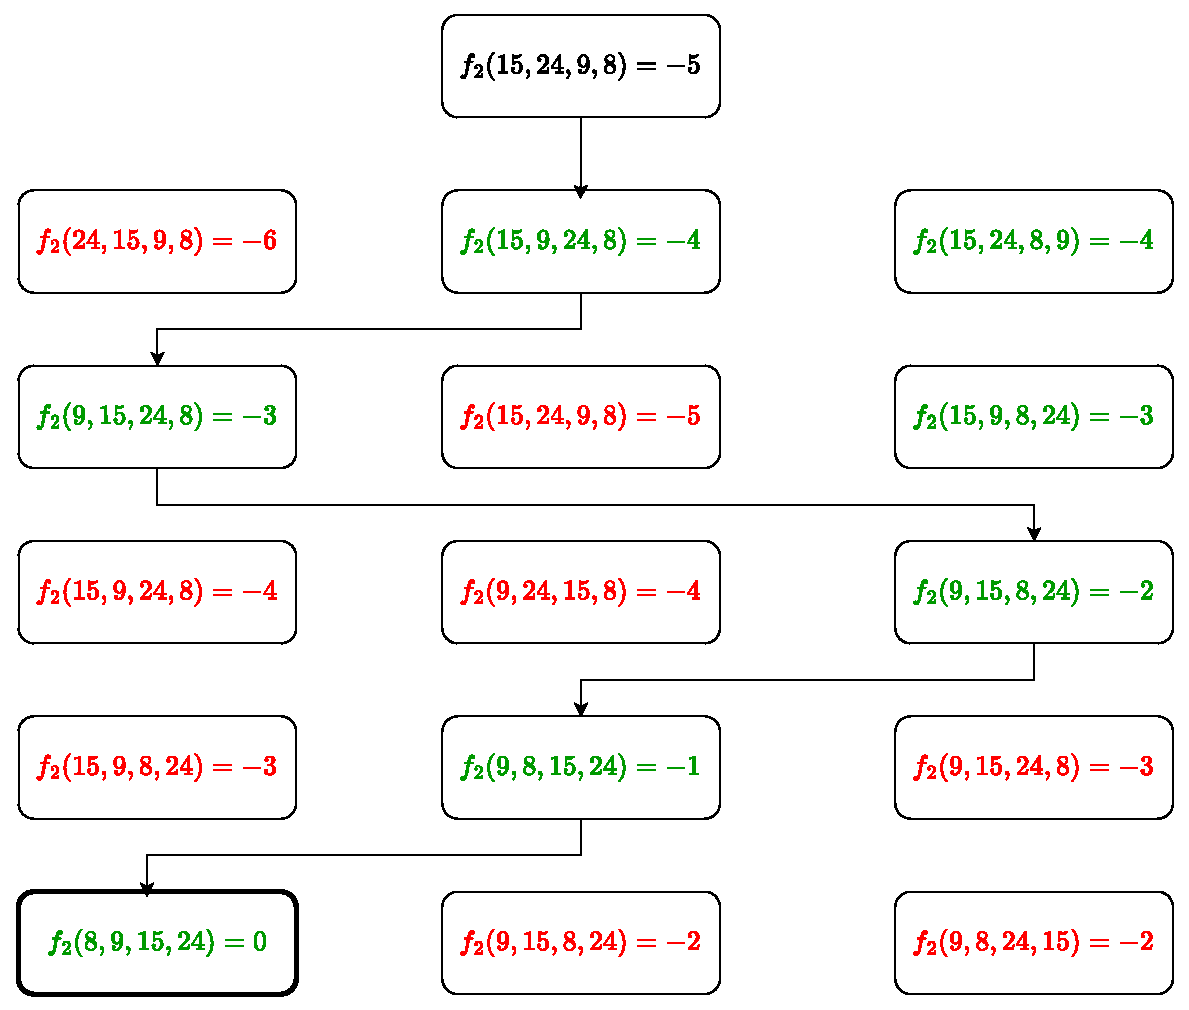
\includegraphics[width=0.7\textwidth]{assets/hill_climbing.pdf}
    \vspace{0.4cm}
    \label{fig:hill climbing}
\end{figure}
به علت ویژگی \lr{involution} اکشن‌ها در این مسئله که اگر یک اکشن را دو بار به صورت متوالی روی یک حالت انجام دهیم دوباره به حالت اولیه برمی‌گردیم، همواره یکی از همسایه‌های تولید شده \lr{fitness} بدتری نسبت به حالت فعلی دارد و می‌توانستیم اصلا آن را تولید نکنیم. \\
همچنین همان طور که در قسمت قبل اشاره شد، هر اکشن میزان \lr{fitness} را تنها یک واحد تغییر می‌دهد، و از طرفی نقطه بهینه محلی غیرسراسری هم نداریم. پس می‌توانیم در هر مرحله یک نابجایی بین دو عضو متوالی را پیدا کرده و آنها را \lr{swap} کنیم. در این صورت دیگر نیازی به تولید همه همسایه‌ها نبود.

\pagebreak

\item الگوریتم \lr{Simulated Annealing} را اجرا می‌کنیم:
\begin{itemize}
    \item \textbf{مرحله 1 ($t=1$)}:
          \begin{itemize}
              \item \textbf{حالت فعلی:} $\pi = (15, 24, 9, 8)$ | $T = 5$ | $f_2(\pi) = -5$
              \item \textbf{همسایه ($swap(1)$):} $\pi' = (24, 15, 9, 8)$ | $f_2(\pi') = -6$
                    \begin{itemize}
                        \item $\Delta E = f_2(\pi') - f_2(\pi) = (-6) - (-5) = -1$
                        \item محاسبه احتمال پذیرش: $P = e^{\Delta E / T} = e^{-1/5} \approx 0.818$
                        \item عدد تصادفی مصرف شده: $r = 0.27$
                        \item \textbf{نتیجه:} چون $r \le P$، این همسایه پذیرفته می‌شود.
                    \end{itemize}
          \end{itemize}

          \vspace{0.7cm}

    \item \textbf{مرحله 2 ($t=2$)}:
          \begin{itemize}
              \item \textbf{حالت فعلی:} $\pi = (24, 15, 9, 8)$ | $T = 4$ | $f_2(\pi) = -6$
              \item \textbf{همسایه ($swap(1)$):} $\pi' = (15, 24, 9, 8)$ | $f_2(\pi') = -5$
                    \begin{itemize}
                        \item $\Delta E = f_2(\pi') - f_2(\pi) = (-5) - (-5) = 1$
                        \item \textbf{نتیجه:} این همسایه بهتر از حالت فعلی بوده و انتخاب می‌شود.
                    \end{itemize}
          \end{itemize}

          \vspace{0.7cm}

    \item \textbf{مرحله 3 ($t=3$)}:
          \begin{itemize}
              \item \textbf{حالت فعلی:} $\pi = (15, 24, 9, 8)$ | $T = 3$ | $f_2(\pi) = -5$
              \item \textbf{همسایه ($swap(1)$):} $\pi' = (24, 15, 9, 8)$ | $f_2(\pi') = -6$
                    \begin{itemize}
                        \item $\Delta E = f_2(\pi') - f_2(\pi) = (-6) - (-5) = -1$
                        \item محاسبه احتمال پذیرش: $P = e^{\Delta E / T} = e^{-1/3} \approx 0.716$
                        \item عدد تصادفی مصرف شده: $r = 0.66$
                        \item \textbf{نتیجه:} چون $r \le P$، این همسایه پذیرفته می‌شود.
                    \end{itemize}
          \end{itemize}

          \vspace{0.7cm}

    \item \textbf{مرحله 4 ($t=4$)}:
          \begin{itemize}
              \item \textbf{حالت فعلی:} $\pi = (24, 15 9, 8)$ | $T = 2$ | $f_2(\pi) = -6$
              \item \textbf{همسایه ($swap(1)$):} $\pi' = (15, 24, 9, 8)$ | $f_2(\pi') = -5$
                    \begin{itemize}
                        \item $\Delta E = f_2(\pi') - f_2(\pi) = (-5) - (-6) = 1$
                        \item \textbf{نتیجه:} این همسایه بهتر از حالت فعلی بوده و انتخاب می‌شود.
                    \end{itemize}
          \end{itemize}

          \vspace{0.7cm}

    \item \textbf{مرحله 5 ($t=5$)}:
          \begin{itemize}
              \item \textbf{حالت فعلی:} $\pi = (15, 24, 9, 8)$ | $T = 1$ | $f_2(\pi) = -5$
              \item \textbf{همسایه ($swap(1)$):} $\pi' = (24, 15, 9, 8)$ | $f_2(\pi') = -6$
                    \begin{itemize}
                        \item $\Delta E = f_2(\pi') - f_2(\pi) = (-6) - (-5) = -1$
                        \item محاسبه احتمال پذیرش: $P = e^{\Delta E / T} = e^{-1/1} \approx 0.367$
                        \item عدد تصادفی مصرف شده: $r = 0.91$
                        \item \textbf{نتیجه:} چون $r > P$، این همسایه پذیرفته نمی‌شود و در مرحله بعد، همسایه بعدی را بررسی می‌کنیم.
                    \end{itemize}
          \end{itemize}

          \vspace{0.7cm}

    \item \textbf{مرحله 6 ($t=6$)}:
          \begin{itemize}
              \item \textbf{حالت فعلی:} $\pi = (15, 24, 9, 8)$ | $T = 0$ | $f_2(\pi) = -5$
              \item \textbf{همسایه ($swap(2)$):} $\pi' = (15, 9, 24, 8)$ | $f_2(\pi') = -4$
                    \begin{itemize}
                        \item $\Delta E = f_2(\pi') - f_2(\pi) = (-4) - (-5) = 1$
                        \item \textbf{نتیجه:} این همسایه بهتر است و انتخاب می‌شود.
                    \end{itemize}
          \end{itemize}

          \vspace{0.7cm}

    \item \textbf{مرحله 7 ($t=7$)}:
          \begin{itemize}
              \item \textbf{حالت فعلی:} $\pi = (15, 9, 24, 8)$ | $T = 0$ | $f_2(\pi) = -4$
              \item \textbf{همسایه ($swap(1)$):} $\pi' = (9, 15, 24, 8)$ | $f_2(\pi') = -3$
                    \begin{itemize}
                        \item $\Delta E = f_2(\pi') - f_2(\pi) = (-3) - (-4) = 1$
                        \item \textbf{نتیجه:} این همسایه بهتر است و انتخاب می‌شود.
                    \end{itemize}
          \end{itemize}

          \vspace{0.7cm}

    \item \textbf{مرحله 8 ($t=8$)}:
          \begin{itemize}
              \item \textbf{حالت فعلی:} $\pi = (9, 15, 24, 8)$ | $T = 0$ | $f_2(\pi) = -3$
              \item \textbf{همسایه ($swap(1)$):} $\pi' = (15, 9, 24, 8)$ | $f_2(\pi') = -4$
                    \begin{itemize}
                        \item $\Delta E = f_2(\pi') - f_2(\pi) = (-4) - (-3) = -1$
                        \item \textbf{نتیجه:} در این مرحله $T=0$ بنابراین همسایه بدتر انتخاب نمی‌شود.
                    \end{itemize}
          \end{itemize}

          \vspace{0.7cm}
\end{itemize}

الگوریتم بدون رسیدن به حالت هدف، خاتمه یافت.

\end{ابجد}
\clearpage

\question{}

در هر گام، مسیرهای فعلی موجود در \lr{fringe} و مسیری که در آن گام از خارج می‌شود را مشخص می‌کنیم.

\begin{itemize}
    \item جستجوی \lr{BFS}:
          \begin{table}[h]
              \centering
              \renewcommand{\arraystretch}{1.5}

              \begin{LTR}
                  \begin{tabular}{|c|>{\raggedright\arraybackslash}p{12cm}|}
                      \hline
                      \lr{step} & \lr{Fringe}                                                                          \\
                      \hline
                      1         & \lr{\textbf{(S)}}                                                                    \\
                      \hline
                      2         & \lr{\sout{(S)}, \textbf{(SA)}, (SB), (SG)}                                           \\
                      \hline
                      3         & \lr{\sout{(S)}, \sout{(SA)}, \textbf{(SB)}, (SG), (SAC), (SAD)}                      \\
                      \hline
                      4         & \lr{\sout{(S)}, \sout{(SA)}, \sout{(SB)}, \textbf{(SG)}, (SAC), (SAD), (SBD), (SBE)} \\
                      \hline
                  \end{tabular}
              \end{LTR}

          \end{table} \\
          خروجی الگوریتم، مسیر $SG$ هست.

          \vspace{1.0cm}

    \item جستجوی \lr{DFS}:
          \begin{table}[h]
              \centering
              \renewcommand{\arraystretch}{1.5}

              \begin{LTR}
                  \begin{tabular}{|c|>{\raggedright\arraybackslash}p{12cm}|}
                      \hline
                      \lr{step} & \lr{Fringe}                                                                    \\
                      \hline
                      1         & \lr{\textbf{(S)}}                                                              \\
                      \hline
                      2         & \lr{\sout{(S)}, (SG), (SB), \textbf{(SA)}}                                     \\
                      \hline
                      3         & \lr{\sout{(S)}, (SG), (SB), \sout{(SA)}, (SAD), \textbf{(SAC)}}                \\
                      \hline
                      4         & \lr{\sout{(S)}, (SG), (SB), \sout{(SA)}, (SAD), \sout{(SAC)}, \textbf{(SACG)}} \\
                      \hline
                  \end{tabular}
              \end{LTR}

          \end{table} \\
          خروجی الگوریتم، مسیر $SACG$ است.

          \pagebreak

    \item جستجوی \lr{UCS}:
          \begin{table}[h]
              \centering
              \renewcommand{\arraystretch}{1.5}

              \begin{LTR}
                  \begin{tabular}{|c|>{\raggedright\arraybackslash}p{12cm}|}
                      \hline
                      \lr{step} & \lr{Fringe}                                                                                                                                         \\
                      \hline
                      1         & \lr{\textbf{(S0)}}                                                                                                                                  \\
                      \hline
                      2         & \lr{\sout{(S0)}, (SA2), \textbf{(SB1)}, (SG9)}                                                                                                      \\
                      \hline
                      3         & \lr{\sout{(S0)}, \textbf{(SA2)}, \sout{(SB1)}, (SG9), (SBD3), (SBE5)}                                                                               \\
                      \hline
                      4         & \lr{\sout{(S0)}, \sout{(SA2)}, \sout{(SB1)}, (SG9), \textbf{(SBD3)}, (SBE5), (SAC4), (SAD5)}                                                        \\
                      \hline
                      5         & \lr{\sout{(S0)}, \sout{(SA2)}, \sout{(SB1)}, (SG9), \sout{(SBD3)}, (SBE5), \textbf{(SAC4)}, (SAD5), (SBDG7)}                                        \\
                      \hline
                      6         & \lr{\sout{(S0)}, \sout{(SA2)}, \sout{(SB1)}, (SG9), \sout{(SBD3)}, (SBE5), \sout{(SAC4)}, \textbf{(SAD5)}, (SBDG7), (SACG8)}                        \\
                      \hline
                      7         & \lr{\sout{(S0)}, \sout{(SA2)}, \sout{(SB1)}, (SG9), \sout{(SBD3)}, \textbf{(SBE5)}, \sout{(SAC4)}, \sout{(SAD5)}, (SBDG7), (SACG8), (SADG9)}        \\
                      \hline
                      8         & \lr{\sout{(S0)}, \sout{(SA2)}, \sout{(SB1)}, (SG9), \sout{(SBD3)}, \sout{(SBE5)}, \sout{(SAC4)}, \sout{(SAD5)}, \textbf{(SBDG7)}, (SACG8), (SADG9)} \\
                      \hline
                  \end{tabular}
              \end{LTR}

          \end{table} \\
          الگوریتم \lr{UCS}، مسیر بهینه $SBDG$ را انتخاب می‌کند.

          \vspace{1.0cm}

    \item جستجوی \lr{Greedy}:
          \begin{table}[h]
              \centering
              \renewcommand{\arraystretch}{1.5}

              \begin{LTR}
                  \begin{tabular}{|c|>{\raggedright\arraybackslash}p{12cm}|}
                      \hline
                      \lr{step} & \lr{Fringe}                                                           \\
                      \hline
                      1         & \lr{\textbf{(S6)}}                                                    \\
                      \hline
                      2         & \lr{\sout{(S6)}, \textbf{(SA0)}, (SB6), (SG0)}                        \\
                      \hline
                      3         & \lr{\sout{(S6)}, \sout{(SA0)}, (SB6), \textbf{(SG0)}, (SAC4), (SAD1)} \\
                      \hline
                  \end{tabular}
              \end{LTR}

          \end{table} \\
          الگوریتم \lr{Greedy} به سرعت مسیر $SG$ را انتخاب می‌کند، که لزوما انتخاب بهینه نیست.

          \pagebreak

    \item جستجوی درختی \lr{A$^*$}:
          \begin{table}[h]
              \centering
              \renewcommand{\arraystretch}{1.5}

              \begin{LTR}
                  \begin{tabular}{|c|>{\raggedright\arraybackslash}p{12cm}|}
                      \hline
                      \lr{step} & \lr{Fringe}                                                                                                                                                 \\
                      \hline
                      1         & \lr{\textbf{(S 0+6)}}                                                                                                                                       \\
                      \hline
                      2         & \lr{\sout{(S 0+6)}, \textbf{(SA 2+0)}, (SB 1+6), (SG 9+0)}                                                                                                  \\
                      \hline
                      3         & \lr{\sout{(S 0+6)}, \sout{(SA 2+0)}, (SB 1+6), (SG 9+0), (SAC 4+4), \textbf{(SAD 5+1)}}                                                                     \\
                      \hline
                      4         & \lr{\sout{(S 0+6)}, \sout{(SA 2+0)}, \textbf{(SB 1+6)}, (SG 9+0), (SAC 4+4), \sout{(SAD 5+1)}, (SADG 9+0)}                                                  \\
                      \hline
                      5         & \lr{\sout{(S 0+6)}, \sout{(SA 2+0)}, \sout{(SB 1+6)}, (SG 9+0), (SAC 4+4), \sout{(SAD 5+1)}, (SADG 9+0), \textbf{(SBD 3+1)}, (SBE 5+10)}                    \\
                      \hline
                      6         & \lr{\sout{(S 0+6)}, \sout{(SA 2+0)}, \sout{(SB 1+6)}, (SG 9+0), (SAC 4+4), \sout{(SAD 5+1)}, (SADG 9+0), \sout{(SBD 3+1)}, (SBE 5+10), \textbf{(SBDG 7+0)}} \\
                      \hline
                  \end{tabular}
              \end{LTR}

          \end{table} \\
          به علت قابل‌قبول بودن تابع هیوریستیک، همان طور که انتظار داشتیم الگوریتم \lr{A$^*$} مسیر بهینه را پیدا کرد. این الگوریتم از \lr{UCS} سریع‌تر، و از الگوریتم \lr{Greedy} کندتر عمل کرد.

          \vspace{1.0cm}

    \item جستجوی گرافی \lr{A$^*$}:
          \begin{table}[ht]
              \centering
              \renewcommand{\arraystretch}{1.5}
              \begin{LTR}
                  \begin{tabular}{|c|>{\raggedright\arraybackslash}p{8cm}|>{\raggedright\arraybackslash}p{3.5cm}|}
                      \hline
                      \lr{step} & \lr{Fringe}                                                                                                                                                        & \textbf{\lr{Closed}}   \\
                      \hline
                      1         & \lr{\textbf{(S 0+6)}}                                                                                                                                              & \lr{\{ \}}             \\
                      \hline
                      2         & \lr{\sout{(S 0+6)}, \textbf{(SA 2+0)}, (SB 1+6), (SG 9+0)}                                                                                                         & \lr{\{S\}}             \\
                      \hline
                      3         & \lr{\sout{(S 0+6)}, \sout{(SA 2+0)}, (SB 1+6), (SG 9+0), (SAC 4+4), \textbf{(SAD 5+1)}}                                                                            & \lr{\{S, A\}}          \\
                      \hline
                      4         & \lr{\sout{(S 0+6)}, \sout{(SA 2+0)}, \textbf{(SB 1+6)}, (SG 9+0), (SAC 4+4), \sout{(SAD 5+1)}, (SADG 9+0)}                                                         & \lr{\{S, A, D\}}       \\
                      \hline
                      5         & \lr{\sout{(S 0+6)}, \sout{(SA 2+0)}, \sout{(SB 1+6)}, (SG 9+0), (SAC 4+4), \sout{(SAD 5+1)}, (SADG 9+0), \textbf{(SBD 3+1)}, (SBE 5+10)}                           & \lr{\{S, A, D, B\}}    \\
                      \hline
                      6         & \lr{\sout{(S 0+6)}, \sout{(SA 2+0)}, \sout{(SB 1+6)}, (SG 9+0), \textbf{(SAC 4+4)}, \sout{(SAD 5+1)}, (SADG 9+0), \sout{(SBD 3+1)}, (SBE 5+10)}                    & \lr{\{S, A, D, B\}}    \\
                      \hline
                      7         & \lr{\sout{(S 0+6)}, \sout{(SA 2+0)}, \sout{(SB 1+6)}, (SG 9+0), \sout{(SAC 4+4)}, \sout{(SAD 5+1)}, (SADG 9+0), \sout{(SBD 3+1)}, (SBE 5+10), \textbf{(SACG 8+0)}} & \lr{\{S, A, D, B, C\}} \\
                      \hline
                  \end{tabular}
              \end{LTR}
          \end{table} \\
          چون $D$ از قبل در \lr{Closed Set} بود، الگوریتم مسیر $SBD$ را بسط نداد، و در نهایت یک مسیر غیربهینه را پیدا کرد.


\end{itemize}

\clearpage

\question{}

\begin{ابجد}
\item طبق تعریف تابع \lr{fitness} در این مسئله داریم:
\begin{align*}
    f(x_1) = 2(5) + (2) + 3(3) - (6) + 2(4) + (1) = 24 \\
    f(x_2) = 2(8) + (1) + 3(7) - (2) + 2(0) + (3) = 39 \\
    f(x_3) = 2(4) + (6) + 3(9) - (1) + 2(2) + (5) = 49 \\
    f(x_4) = 2(9) + (0) + 3(2) - (5) + 2(7) + (8) = 41
\end{align*}
بر اساس مقادیر \lr{fitness} محاسبه شده، مشاهده می‌شود که $x_3$ بهترین عضو در جمعیت اولیه است.

\item عملیات تقاطع (\lr{Crossover}) به این شکل است:
\begin{figure}[htpb]
    \centering
    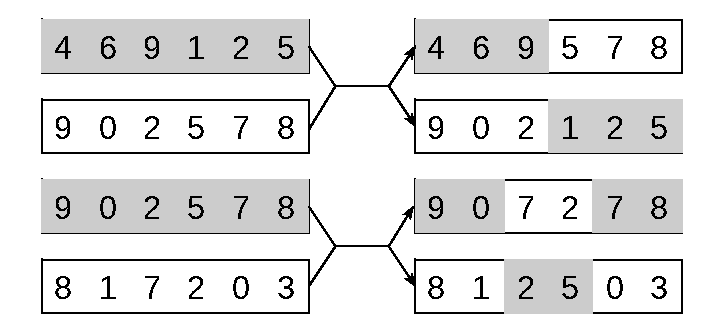
\includegraphics[width=0.5\textwidth]{assets/crossover_diagram.pdf}
    \label{fig:crossover}
\end{figure}

\item عملیات جهش را مطابق با صورت سوال انجام می‌دهیم:
\begin{figure}[htpb]
    \centering
    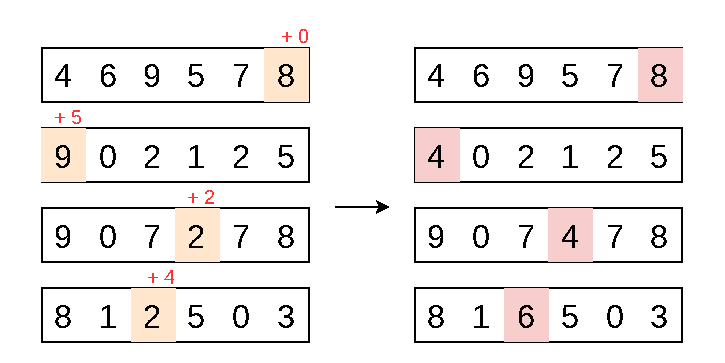
\includegraphics[width=0.5\textwidth]{assets/mutation_diagram.pdf}
    \label{fig:mutation}
\end{figure}

\item ابتدا \lr{fitness} جمعیت جدید را محاسبه می‌کنیم:
\begin{align*}
    f(x_1') = 2(4) + (6) + 3(9) - (5) + 2(7) + (8) = 58 \\
    f(x_2') = 2(4) + (0) + 3(2) - (1) + 2(2) + (5) = 22 \\
    f(x_3') = 2(9) + (0) + 3(7) - (4) + 2(7) + (8) = 57 \\
    f(x_4') = 2(8) + (1) + 3(6) - (5) + 2(0) + (3) = 33
\end{align*}
میانگین جمعیت اولیه و جمعیت جدید را محاسبه می‌کنیم:
\begin{align*}
    \overline{f(x)}  & = \frac{24+39+49+41}{4} = 38.25 \\
    \overline{f(x')} & = \frac{58+22+57+33}{4} = 42.5
\end{align*}
همان طور که انتظار داشتیم، مشاهده می‌شود که میانگین \lr{fitness} در جمعیت جدید بیشتر از جمعیت اولیه است.

\end{ابجد}
\clearpage

\question{}
\begin{ابجد}
\item مسئله را به این شکل تعریف می‌کنیم:
\begin{itemize}
    \item \textbf{حالت‌ها}: می‌توانیم لیوان‌ها را در حالت کامل شماره‌گذاری کنیم (مثلا با شروع از ردیف پایین، و در هر ردیف از چپ به راست). در این صورت هر حالت، مجموعه لیوان‌هایی است که باقی مانده‌اند؛ بدیهی است که هر حالت زیرمجموعه حالت اولیه محسوب می‌شود.
    \item \textbf{کنش‌ها}: ضربه زدن به هر لیوانی در حالت فعلی که حداکثر یک لیوان به طور مستقیم روی آن قرار گرفته، و انداختن آن لیوان و تمام لیوان‌هایی که به طور مستقیم و غیرمستقیم بالای آن قرار گرفتند. (با توجه به محدودیت اعمال شده در انتخاب لیوان، نمی‌توانیم به لیوان‌هایی که دو لیوان روی آنها قرار گرفته ضربه بزنیم.)
    \item \textbf{هزینه کنش‌ها}: هزینه تمام کنش‌ها را مساوی و برابر با 1 در نظر می‌گیریم.
    \item \textbf{حالت(های) هدف}: هر مجموعه‌ای از لیوان‌ها که تعداد لیوان‌های ریخته شده در آن بیشتر از نصف کل لیوان‌های حالت اولیه باشد، حالت هدف محسوب می‌شود. (با این تعریف بعضی از حالت‌های هدف، ممکن نیستند؛ به عنوان مثال حالت $\{1, 2, 3, 4, 5, 7, 8, 9, 10\}$ را برای مسئله ترسیم شده در صورت سوال در نظر بگیرید. این حالت از دو نظر مشکل دارد: اول اینکه در حالت اولیه دو لیوان به طور مستقیم روی لیوان 6 قرار گرفته‌اند و نمی‌توانیم به آن ضربه بزنیم. همچنین اگر فرض کنیم به این لیوان ضربه زده باشیم، لیوان‌های 8، 9 و 10 گه به طور مستقیم و غیرمستقیم روی آن قرار دارند هم باید حذف می‌شدند. پس این حالت هدف قابل دستیابی نیست.)

\end{itemize}

\item اگر بخواهیم در هر مرحله تعداد لیوان‌هایی که ریخته می‌شوند را بیشینه کنیم، در حالت اولیه باید به راست‌ترین یا چپ‌ترین لیوان ردیف پایین ضربه بزنیم. هر مورد را جداگانه بررسی می‌کنیم:
\begin{itemize}
    \item \textbf{قابل قبول بودن}: با ارائه مثال نقض، نشان می‌دهیم که تابع $h$ قابل قبول نیست. \\
          فرض کنید در ابتدا یک هرم کامل با ارتفاع 14 داریم. این هرم در کل $\frac{14 \times 15}{2} = 105$ لیوان دارد. پس باید حداقل 53 لیوان بیفتند. حال فرض کنید تعدادی از لیوان‌ها را حذف کردیم و در نهایت به حالت زیر رسیدیم:
          \begin{figure}[H]
              \centering
              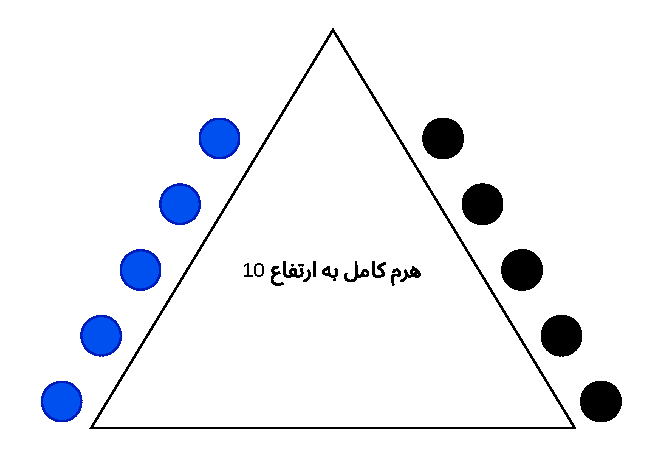
\includegraphics[width=0.5\textwidth]{assets/6_b_0.pdf}
          \end{figure}

          بهترین انتخاب در این حالت، انتخاب یکی از دو لیوان کناری در پایین‌ترین لایه هست، که در این صورت 5 لیوان فرومی‌ریزند. پس $\displaystyle \max_{c \in \text{targetable cups}(S)} f(c) = 5$.
          در این حالت $\frac{10 \times 11}{2} + 10 = 65$ لیوان داریم، پس $105 - 65 = 40$ لیوان تا الان افتاده‌اند و باید $53-40=13$ لیوان دیگر را بیندازیم. پس:
          \begin{equation*}
              h(S) = \frac{13}{5} = 2.6
          \end{equation*}
          حال فرض کنید یکی از دو لیوان مورد نظر را هدف قرار دهیم. سپس، می‌توانیم یکی از لیوان‌های کناری در لایه پایین هرم 10 تایی را هدف قرار دهیم. در این صورت 10 لیوان می‌افتند؛ در کل 55 لیوان تا الان افتاده‌اند و به حالت هدف رسیده‌ایم.
          \begin{equation*}
              h(S) = 2.6 \nleq h^*(S) = 2
          \end{equation*}
          پس تابع $h$ قابل قبول نیست.

    \item \textbf{یک‌نوا بودن}: با یک مثال نقض، نشان می‌دهیم که تابع مورد نظر یک‌نوا نیست. \\
          فرض کنید در ابتدا یک هرم کامل با ارتفاع 5 داریم:
          \begin{figure}[H]
              \centering
              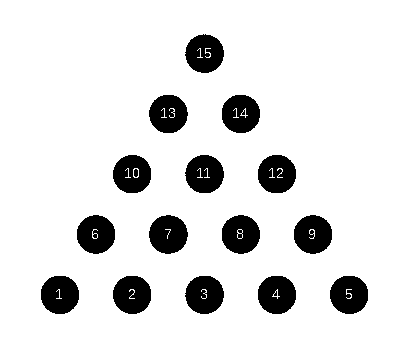
\includegraphics[width=0.5\textwidth]{assets/6_b_1.pdf}
          \end{figure}

          در هرم کامل، $\frac{5 \times 6}{2} = 15$ لیوان داریم و باید حداقل 8 لیوان فرو بریزند. فرض کنید 5 تا از لیوان‌های بالا حذف شده‌اند و به این حالت رسیدیم:
          \begin{figure}[H]
              \centering
              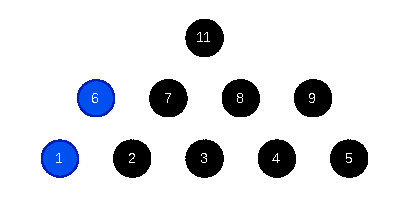
\includegraphics[width=0.5\textwidth]{assets/6_b_2.pdf}
          \end{figure}

          مقدار $\displaystyle \max_{c \in \text{targetable cups}(S)} f(c)$ در این حالت، به ازای لیوان شماره 1 (یا لیوان شماره 5) رخ می‌دهد که با ضربه زدن به آن، دو لیوان فرو می‌ریزند. (توجه کنید که در این حالت نمی‌توانیم لیوان‌های شماره 2 یا 4 را هدف قرار دهیم) بنابراین مقدار تابع $h$ در این حالت برابر است با:
          \begin{equation*}
              h(S) = \frac{3}{2}
          \end{equation*}
          به توپ شماره 1 ضربه زده (این اکشن هزینه 1 دارد) و به این حالت می‌رسیم:
          \begin{figure}[H]
              \centering
              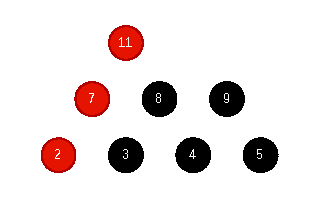
\includegraphics[width=0.5\textwidth]{assets/6_b_3.pdf}
          \end{figure}

          اکنون که یکی از لیوان‌های روی لیوان شماره 2 افتاده، می‌توانیم این لیوان را هدف قرار دهیم که در این صورت 3 لیوان می‌افتند. پس در این حالت:
          \begin{equation*}
              h(S') = \frac{1}{3}
          \end{equation*}

          داریم:
          \begin{equation*}
              h(S) - h(S') = \frac{3}{2} - \frac{1}{3} = \frac{7}{6} \nleq \mathrm{cost}(S \to S') = 1
          \end{equation*}
          بنابراین تابع $h$ یک‌نوا نیست.
\end{itemize}

\item تابع اکتشافی $h'$ را به این شکل تعریف می‌کنیم:
\begin{align*}
    h'(S) = \begin{cases}
                2   & \text{\lr{S} حالت اولیه باشد} \\
                0   & \text{\lr{S} حالت هدف باشد}   \\
                0.5 & \text{حالت‌های دیگر}
            \end{cases}
\end{align*}

برای اثبات قابل قبول بودن $h'$ باید نشان دهیم:
\begin{equation*}
    \forall S : 0 \leq h'(S) \leq h^*(S)
\end{equation*}
برای حالت‌هایی به جز حالت اولیه، بدیهی است که این رابطه صحیح می‌باشد. \\
اگر ارتفاع هرم $n$ باشد، در کل $\frac{n(n+1)}{2}$ لیوان داریم و باید حداقل $\lfloor \frac{n(n+1)}{4} + 1 \rfloor$ لیوان فرو بریزند. همچنین در هر حالت، حداکثر $n$ لیوان را می‌توانیم بیندازیم، که البته می‌دانیم این کار تنها در یک حرکت ممکن است. پس:
\begin{equation*}
    h^*(S_0) \geq \frac{\lfloor \frac{n(n+1)}{4} + 1 \rfloor}{n} > \frac{\frac{n(n+1)}{4}}{n} = \frac{n+1}{4}
\end{equation*}
که $S_0$ حالت اولیه است. با فرض اینکه ارتفاع هرم اولیه حداقل 15 باشد، داریم $h^*(S_0) \geq 4$ و در نتیجه $h'(S_0) < h^*(S_0)$. \\
پس تابع $h'$ قابل قبول است. \\

برای نشان دادن اینکه این تابع یک‌نوا نیست، کافی است مثالی را تصور کنیم که از حالت اولیه $S_0$ به حالت $S$ می‌رویم. ($S$ حالت هدف نیست)
\begin{equation*}
    h'(S_0) - h'(S) = 2 - 0.5 = 1.5 \nleq  \mathrm{cost}(S_0 \to S) = 1
\end{equation*}
پس تابع اکتشافی $h'$، یک‌نوا نیست.

\end{ابجد}

\end{document}
